% Chapter on modal logic. Original author: Rob Trueman, York
% University, http://www.rtrueman.com/

\part{Modal logic}
\label{ch.ML}
\addtocontents{toc}{\protect\mbox{}\protect\hrulefill\par}

%\usepackage{gensymb}
%\input{fitch1.sty}

\chapter{Introducing Modal Logic}
\label{Intro}

Modal Logic (ML) is the logic of \emph{necessity} and \emph{possibility}. We use $\Box$ to express necessity, and $\Diamond$ to express possibility. So you can read $\Box \meta{A}$ as \emph{It is necessarily the case that} $\meta{A}$, and $\Diamond \meta{A}$ as \emph{It is possibly the case that} $\meta{A}$.

There are lots of different kinds of necessity. It is \emph{humanly impossible} for me to run at 100mph. Given the sorts of creatures that we are, no human can do that. But still, it isn't \emph{physically impossible} for me to run that fast. We haven't got the technology to do it yet, but it is surely physically possible to swap my biological legs for robotic ones which could run at 100mph. By contrast, it is physically impossible for me to run faster than the speed of light. The laws of physics forbid any object from accelerating up to that speed. But even that isn't \emph{logically} impossible. It isn't a contradiction to imagine that the laws of physics might have been different, and that they might have allowed objects to move faster than light.

So, there are lots of kinds of necessity. Which kind does ML deal with? \emph{All of them!} ML is a very flexible tool. We start with a basic set of rules that govern $\Box$ and $\Diamond$, and then add more rules to fit whatever kind of necessity we are interested in. In fact, ML is so flexible that we do not even have to think of $\Box$ and $\Diamond$ as expressing \emph{necessity} and \emph{possibility}. We might instead read $\Box$ as expressing \emph{provability}, so that $\Box\meta{A}$ means \emph{It is provable that} $\meta{A}$, and $\Diamond\meta{A}$ means \emph{It is not refutable that} $\meta{A}$. Or we might read $\Box$ as expressing \emph{moral obligation}, so that $\Box \meta{A}$ means \emph{It is morally obligatory that} $\meta{A}$, and $\Diamond \meta{A}$ means \emph{It is morally permissible that} $\meta{A}$. All we would need to do is cook up the right rules for these different readings of $\Box$ and $\Diamond$.

But, having said all of that, in this module we will be primarily concerned with necessity and possibility, and so for the most part, that is how we will think of $\Box$ and $\Diamond$.


\section*{Further reading}
\begin{itemize}
\item Hughes, G.E., \& Cresswell, M.J. (1996) \emph{A New Introduction to Modal Logic}, Oxford: Routledge.
\item Priest, G. (2008) \emph{An Introduction to Non-Classical Logic}, 2nd ed., Cambridge: Cambridge University Press.
\item Garson, J.W. (2013) \emph{Modal Logic for Philosophers}, 2nd ed., Cambridge: Cambridge University Press.
\end{itemize}



\chapter{The Language of ML}
\label{TFLtoML}

We have two aims in this little primer. First, we want to learn how to prove things in ML. Second, we want to see how to construct interpretations for ML. But before we can do either of these things, we need to explain how to construct sentences in ML.

The language of ML is an extension of TFL, as explained in \emph{forall}$\meta{x}$. We could have started with FOL, which would have given us Quantified Modal Logic (QML). QML is much more powerful than ML, but it is also much, much more complicated. So we are going to keep things simple, and start with TFL.

Just like TFL, ML starts with an infinite stock of \emph{atoms}. These are written as capital letters, with or without numerical subscripts: $A$, $B$, \dots  $A_1$, $B_1$, \dots  We then take all of the rules about how to make sentences from TFL, and add two more for $\Box$ and $\Diamond$:
\begin{itemize}
\item[(1)]Every atom of ML is a sentence of ML.
\item[(2)]If $\meta{A}$ is a sentence of ML, then $\enot\meta{A}$ is a sentence of ML.
\item[(3)]If $\meta{A}$ and $\meta{B}$ are sentences of ML, then $(\meta{A}\eand\meta{B})$ is a sentence of ML.
\item[(4)]If $\meta{A}$ and $\meta{B}$ are sentences of ML, then $(\meta{A}\eor\meta{B})$ is a sentence of ML.
\item[(5)]If $\meta{A}$ and $\meta{B}$ are sentences of ML, then $(\meta{A}\eif\meta{B})$ is a sentence of ML.
\item[(6)]If $\meta{A}$ and $\meta{B}$ are sentences of ML, then $(\meta{A}\eiff\meta{B})$ is a sentence of ML.
\item[(7)]If $\meta{A}$ is a sentence of ML, then $\Box\meta{A}$ is a sentence of ML.
\item[(8)]If $\meta{A}$ is a sentence of ML, then $\Diamond\meta{A}$ is a sentence of ML.
\item[(9)]Nothing else is a sentence of ML.
\end{itemize}
Here are some examples of ML sentences:
\begin{itemize}
\item[]$A,\;P\eor Q,\;\Box A,\;C\eor \Box D,\;\Box\Box (A\eif R),\;\Box\Diamond (S\eand (Z\eiff (\Box W \eor \Diamond Q)))$
\end{itemize}

\chapter{Natural Deduction for ML}
\label{Proof}

Now that we know how to make sentences in ML, we can look at how to \emph{prove} things in ML. Just as in \emph{forall}$\meta{x}$, we will use $\vdash$ to express provability.  So $\meta{A}_1,\meta{A}_2, \dots \meta{A}_n \vdash \meta{C}$ means that $\meta{C}$ can be proven from $\meta{A}_1,\meta{A}_2, \dots \meta{A}_n$. However, we will be looking at a number of different systems of ML, and so it will be useful to add a subscript to indicate which system we are working with. So for example, if we want to say that we can prove $\meta{C}$ from $\meta{A}_1,\meta{A}_2, \dots \meta{A}_n$ \emph{in system} $K$, we will write: $\meta{A}_1,\meta{A}_2, \dots \meta{A}_n \vdash_K \meta{C}$.

\section{System $K$}
\label{K}

We start with a particularly simple system called $K$, in honour of the philosopher and logician Saul Kripke. $K$ includes all of the natural deduction rules from TFL, including the derived rules as well as the basic ones. (I won't go over all of these again here. If you would like a reminder, just look back over \emph{forall}$\meta{x}$!) $K$ then adds two new basic rules. Here is the first rule:
\factoidbox{\[\begin{nd}
\have[m]{m}{\Box (\meta{A}\eif \meta{B})}
\have[\ ]{n}{\Box \meta{A}\eif \Box\meta{B}}\by{Dist}{m}
\end{nd}\]
}

This is called the \emph{Distribution Rule}, because it tells us that $\Box$ `distributes' over $\eif$.

The next rule is a little more complicated. It is known as \emph{Necessitation}, and it is our fundamental method of introducing $\Box$ into proofs. The basic idea is simple enough: if $\meta{A}$ is a theorem, then $\Box \meta{A}$ should be a theorem too. (Remember that to call $\meta{A}$ a theorem is to say that we can prove $\meta{A}$ without relying on any undischarged assumptions.) But figuring out how to actually implement this rule in our proof system is a little tricky.

Suppose we wanted to use Necessitation to prove $\Box(A\eif A)$. The first thing we need to do is prove that $A\eif A$ is a theorem. You already know how to do that using TFL. You simply present a proof of $A\eif A$ which doesn't start with any premises, like this:
\[\begin{nd}
\open
\hypo{1}{A}
\have{2}{A}\by{R}{1}
\close
\have{3}{A\eif A}\by{$\eif$I}{1-2}
\end{nd}\]

\noindent Now that we have proven that $A\eif A$ is a theorem, we should be able to apply Necessitation to infer $\Box(A\eif A)$. And in this case, there is no real problem. We could just extend our proof by one line, like this:
\[\begin{nd}
\open
\hypo{1}{A}
\have{2}{A}\by{R}{1}
\close
\have{3}{A\eif A}\by{$\eif$I}{1-2}
\have{4}{\Box (A\eif A)}\by{Nec}{3}
\end{nd}\]

\noindent But now imagine that we were not just trying to prove that $\Box(A\eif A)$ is a theorem. Imagine instead we were trying to show that $B\vdash_K B\eand \Box(A\eif A)$. We might try something like this:
\[\begin{nd}
\hypo{0}{B}
\open
\hypo{1}{A}
\have{2}{A}\by{R}{1}
\close
\have{3}{A\eif A}\by{$\eif$I}{1-2}
\have{4}{\Box (A\eif A)}\by{Nec}{3}
\have{5}{B\eand\Box (A\eif A)}\by{$\eand$I}{0,4}
\end{nd}\]

\noindent But that is no good. Now our proof starts with an undischarged assumption, $B$, and so line 4 no longer establishes that $A\eif A$ is a \emph{theorem}. It only shows that $B\vdash_K A\eif A$. So we have not shown that the Necessitation step at line 5 is legitimate.

To solve this problem, we need to find some way of showing that $A\eif A$ is a theorem \emph{in the middle of a longer proof}. Here is how we will do that. You are already familiar with the idea that you can trigger a new subproof whenever you like, just by making a new assumption. We will now push that idea a little further, and say that you can also trigger a subproof by making an `empty assumption', like this:
\[\begin{nd}
\hypo{1}{B}
\open
\hypo{2}{\hspace{50pt}}
\open
\hypo{3}{A}
\have{4}{A}\by{R}{3}
\close
\have{5}{A\eif A}\by{$\eif$I}{3-4}
\close
\have{6}{\Box(A\eif A)}\by{Nec}{2-5}
\have{7}{B \eand \Box(A\eif A)}\by{$\eand$I}{1,6}
\end{nd}\]

\noindent When we start a subproof by making an `empty assumption', we are indicating that we are going to use that subproof to show that something is a theorem. We then write out a proof of this theorem within the subproof. So in our case above, we triggered a subproof by making an empty assumption at line 2, and then wrote out our proof that $A\eif A$ is a theorem inside this subproof. After that, we stepped back out of the subproof, and used Necessitation to infer $\Box(A\eif A)$.

Here, then, is our final formulation of the Necessitation Rule:
\factoidbox{
\[\begin{nd}
\open
\hypo[m]{m}{\hspace{50pt}}
\have[n]{n}{\meta{A}}
\close
\have[\,]{o}{\Box\meta{A}}\by{Nec}{m-n}
\end{nd}\]
No line above line $m$ may be cited by any rule within the subproof begun at line $m$.
}

\noindent It is essential to emphasise that if you have trigger a subproof with one of these empty assumptions, then for the duration of that subproof, you cannot use any rule which appeals to anything you proved outside of the subproof. Otherwise, we would get terrible results. For example, we could provide the following proof to vindicate $A\therefore \Box A$:
\[\begin{nd}
\hypo{1}{A}
\open
\hypo{2}{\hspace{50pt}}
\have{3}{A}\by{R}{1}
\close
\have{4}{\Box A}\by{Nec}{2-3}
\end{nd}
\]
This is not a legitimate application of Necessitation, because at line 3 we appealed to line 1, even though line 1 comes before the empty assumption at line 2.

Distribution and Necessitation are the only two basic rules that $K$ adds to TFL. Like I said, $K$ is a very simple system! But $K$ is more powerful than you might have thought. You can prove a fair few things in it.


\section{Possibility}
\label{possibility}

In the last subsection, we looked at all of the basic rules for $K$. But you might have noticed that all of these rules were about necessity, $\Box$, and none of them were about possibility, $\Diamond$. That's because we can \emph{define} possibility in terms of necessity:
\factoidbox{
	$\Diamond\meta{A}=_{df} \enot \Box\enot \meta{A}$
}
In other words, to say that $\meta{A}$ is \emph{possibly true}, is to say that $\meta{A}$ is \emph{not necessarily false}. As a result, it isn't really essential to add a $\Diamond$, a special symbol for possibility, into system $K$. Still, the system will be \emph{much} easier to use if we do, and so we will add the following definitional rules:
\factoidbox{
\[\begin{nd}
\have[m]{m}{\enot\Box\enot \meta{A}}
\have[\, ]{n}{\Diamond \meta{A}}\by{$\Diamond$Def}{m}
\end{nd}
\]
\[\begin{nd}
\have[m]{m}{\Diamond \meta{A}}
\have[\, ]{n}{\enot\Box\enot \meta{A}}\by{$\Diamond$Def}{m}
\end{nd}\]
}
Importantly, you should not think of these rules as any real addition to $K$: they just record the way that $\Diamond$ is defined in terms of $\Box$.

If we wanted, we could leave our rules for $K$ here. But it will be helpful to add some \emph{Modal Conversion} rules, which give us some more ways of flipping between $\Box$ and $\Diamond$:
\factoidbox{
\[\begin{nd}
\have[m]{m}{\enot\Box \meta{A}}
\have[\, ]{n}{\Diamond \enot\meta{A}}\by{MC}{m}
\end{nd}
\]
\[\begin{nd}
\have[m]{m}{\Diamond \enot \meta{A}}
\have[\, ]{n}{\enot\Box \meta{A}}\by{MC}{m}
\end{nd}\]
\[\begin{nd}
\have[m]{m}{\enot\Diamond \meta{A}}
\have[\, ]{n}{\Box \enot\meta{A}}\by{MC}{m}
\end{nd}\]
\[\begin{nd}
\have[m]{m}{\Box\enot \meta{A}}
\have[\, ]{n}{\enot\Diamond\meta{A}}\by{MC}{m}
\end{nd}\]
}
These Modal Conversion Rules are also no addition to the power of $K$, because they can be derived from the basic rules, along with the definition of $\Diamond$. 

The proofs for 6 and 7 show us something important. When laying out system $K$, we started with $\Box$ as our primitive modal symbol, and then defined $\Diamond$ in terms of it. But if we had preferred, we could have started with $\Diamond$ as our primitive, and then defined $\Box$ as follows: $\Box\meta{A} =_{df} \enot \Diamond \enot \meta{A}$. There is, then, no sense in which necessity is somehow more \emph{fundamental} than possibility. Necessity and possibility are exactly as fundamental as each other.

\section{System $T$}
\label{T}

So far we have focussed on $K$, which is a very simple modal system. $K$ is so weak that it will not even let you prove $\meta{A}$ from $\Box\meta{A}$. But if we are thinking of $\Box$ as expressing \emph{necessity}, then we will want to be able to make this inference: if $\meta{A}$ is \emph{necessarily true}, then it must surely be \emph{true}!

This leads us to a new system, $T$, which we get by adding the following rule to $K$:
\factoidbox{
\[\begin{nd}
\have[m]{m}{\Box \meta{A}}
\have[\, ]{n}{\meta{A}}\by{$T$}{m}
\end{nd}\]
}

We can prove things in $T$ which we could not prove in $K$.

\section{System $S4$}
\label{S4}

$T$ allows you to strip away the necessity boxes: from $\Box \meta{A}$, you may infer $\meta{A}$. But what if we wanted to add extra boxes? That is, what if we wanted to go from $\Box\meta{A}$ to $\Box\Box\meta{A}$? Well, that would be no problem, if we had proved $\Box\meta{A}$ by applying Necessitation. For example, we could prove $\Box\Box (P\eif P)$ like this:
\[
\begin{nd}
\open
\hypo{1}{\hspace{50pt}}
\open
\hypo{2}{\hspace{50pt}}
\open
\hypo{3}{P}
\have{4}{P}\by{R}{3}
\close
\have{5}{P\eif P}\by{$\eif$I}{3-4}
\close
\have{6}{\Box(P\eif P)}\by{Nec}{2-5}
\close
\have{7}{\Box\Box(P\eif P)}\by{Nec}{1-6}
\end{nd}
\]
But what if we didn't prove $\Box\meta{A}$ by applying Necessitation? What if $\Box\meta{A}$ were just an assumption we started our proof with? Could we infer $\Box\Box\meta{A}$ then? Not in $T$, we couldn't. And this might well strike you as a limitation of $T$, at least if we are reading $\Box$ as expressing \emph{necessity}. It seems intuitive that if $\meta{A}$ is necessarily true, then it couldn't have \emph{failed} to be necessarily true.

This leads us to another new system, $S4$, which we get by adding the following rule to $T$:
\factoidbox{
\[\begin{nd}
\have[m]{m}{\Box\meta{A}}
\have[\, ]{n}{\Box\Box\meta{A}}\by{$S4$}{m}
\end{nd}\]
}
Now we can prove even more results. 

The proof of 3 shows us that as well as letting us \emph{add} extra \emph{boxes}, $S4$ lets us \emph{delete} extra \emph{diamonds}: from $\Diamond\Diamond \meta{A}$, you can always infer $\Diamond\meta{A}$.

\section{System $S5$}
\label{S5}

In $S4$, we can always add a box in front of another box. But $S4$ does not automatically let us add a box in front of a \emph{diamond}. That is, $S4$ does not generally permit the inference from $\Diamond\meta{A}$ to $\Box\Diamond\meta{A}$. But again, that might strike you as a shortcoming, at least if you are reading $\Box$ and $\Diamond$ as expressing \emph{necessity} and \emph{possibility}. It seems intuitive that if $\meta{A}$ is possibly true, then it couldn't have \emph{failed} to be possibly true.

This leads us to our final modal system, $S5$, which we get by adding the following rule to $T$:
\factoidbox{
\[\begin{nd}
\have[m]{m}{\Diamond \meta{A}}
\have[\, ]{n}{\Box\Diamond\meta{A}}\by{$S5$}{m}
\end{nd}\]
}

This rule allows us to show, for instance, that $\Diamond\Box A\vdash_{S5}\Box A$. So, as well as adding boxes in front of diamonds, we can also delete diamonds in front of boxes. And the proof for 3 shows us something important too. We got $S5$ just by adding a rule to $T$. We did not stop to add the rule from $S4$ to $S5$. However, the proof of 3 shows us that we can derive the $S4$ rule within $S5$. So $S5$ is \emph{stronger} than $S4$: anything that can be proved in $S4$ can be proved in $S5$ too. In fact, $S5$ is \emph{strictly stronger} than $S4$: there are things which can be proved in $S5$, but not in $S4$.

The important point about $S5$ can be put like this: if you have a long string of boxes and diamonds, in any combination whatsoever, you can delete all but the last of them. So for example, $\Diamond\Box\Diamond\Diamond\Box\Box\Diamond\Box A$ can be simplified down to just $\Box A$.

\practiceproblems

\problempart
Provide proofs for the following:
\begin{earg}
\item $\Box (A\eand B)\vdash_K\Box A \eand \Box B$
\item $\Box A\eand\Box B\vdash_K\Box( A \eand  B)$
\item $\Box A\eor\Box B\vdash_K\Box( A \eor  B)$
\item $\Box (A \eiff B)\vdash_K \Box A \eiff \Box B$
\end{earg}

\problempart
Provide proofs for the following (without using Modal Conversion!):
\begin{earg}
\item $\enot\Box A\vdash_K \Diamond \enot A$
\item $\Diamond\enot A\vdash_K\enot \Box A$
\item $\enot\Diamond A\vdash_K\Box\enot A$
\item $\Box\enot A\vdash_K\enot\Diamond A$
\end{earg}

\problempart
Provide proofs of the following (and now feel free to use Modal Conversion!):
\begin{earg}
\item $\Box(A\eif B), \Diamond A \vdash_K \Diamond B$
\item $\Box A \vdash_K \enot\Diamond\enot A$
\item $\enot\Diamond\enot A \vdash_K \Box A$
\end{earg}

\problempart
Provide proofs for the following:
\begin{earg}
\item $P\vdash_T\Diamond P$
\item $\vdash_T (A\eand B)\eor(\enot \Box A\eor\enot\Box B)$
\end{earg}

\problempart
Provide proofs for the following:
\begin{earg}
\item $\Box(\Box A\eif B), \Box (\Box B\eif C), \Box A \vdash_{S4}\Box\Box B \eand \Box\Box\Box C$
\item $\Box A \vdash_{S4} \Box(\Box A \eor B)$
\item $\Diamond \Diamond A \vdash_{S4} \Diamond A$
\end{earg}


\problempart
Provide proofs in $S5$ for the following:
\begin{earg}
\item $\enot\Box\enot A, \Diamond B\vdash_{S5}\Box(\Diamond A \eand \Diamond B)$
\item $\Diamond\Box A\vdash_{S5}\Box A$
\item $\Box A\vdash_{S5}\Box\Box A$
\end{earg}


\chapter{Semantics for ML}
\label{Semantics}

So far, we have focussed on laying out various systems of Natural Deduction for ML. Now we will look at the \emph{semantics} for ML. A semantics for a language is a method for assigning truth-values to the sentences in that language. So a semantics for ML is a method for assigning truth-values to the sentences of ML.

\section{Interpretations of ML}

The big idea behind the semantics for ML is this. In ML, sentences are not just true or false, full stop. A sentence is true or false \emph{at a given possible world}, and a single sentence may well be true at some worlds and false at others. We then say that $\Box \meta{A}$ is true iff $\meta{A}$ is true at \emph{every} world, and $\Diamond\meta{A}$ is true iff $\meta{A}$ is true at \emph{some} world.

That's the big idea, but we need to refine it and make it more precise. To do this, we need to introduce the idea of an \emph{interpretation} of ML. The first thing you need to include in an interpretation is a collection of \emph{possible worlds}. Now, at this point you might well want to ask: What exactly is a possible world? The intuitive idea is that a possible world is another way that this world could have been. But what exactly does that mean? This is an excellent philosophical question, and we will look at it in a lot of detail later. But we do not need to worry too much about it right now. As far as the formal logic goes, possible worlds can be anything you like. All that matters is that you supply each interpretation with a non-empty collection of things labelled \textsc{possible worlds}.

Once you have chosen your collection of possible worlds, you need to find some way of determining which sentences of ML are true at which possible worlds. To do that, we need to introduce the notion of a \emph{valuation function}. Those of you who have studied some maths will already be familiar with the general idea of a function. But for those of you who haven't, a function is a mathematical entity which maps arguments to values. That might sound a little bit abstract, but some familiar examples will help. Take the function $x+1$. This is a function which takes in a number as argument, and then spits out the next number as value. So if you feed in the number 1 as an argument, the function $x+1$ will spit out the number 2 as a value; if you feed in 2, it will spit out 3; if you feed in 3, it will spit out 4 \dots  Or here is another example: the function $x+y$. This time, you have to feed two arguments into this function if you want it to return a value: if you feed in 2 and 3 as your arguments, it spits out 5; if you feed in 1003 and 2005, it spits out 3008; and so on.

A valuation function for ML takes in a sentence and a world as its arguments, and then returns a truth-value as its value. We can use numbers to represent the truth-values: 0 represents falsehood, 1 represents truth. So if $\nu$ is a valuation function and $w$ is a possible world, $\nu_w(\meta{A})$ is whatever truth-value $\nu$ maps $\meta{A}$ and $w$ to: if $\nu_w(\meta{A})=0$, then $\meta{A}$ is false at world $w$ on valuation $\nu$; if $\nu_w(\meta{A})=1$, then $\meta{A}$ is true at world $w$ on valuation $\nu$.

These valuation functions are allowed to map any \emph{atomic} sentence to any truth-value at any world. But there are rules about which truth-values more complex sentences get assigned at a world. Here are the rules for the connectives from TFL:
\begin{itemize}
\item[(1)]$\nu_w(\enot\meta{A})=1$ iff: $\nu_w(\meta{A})=0$
\item[(2)]$\nu_w(\meta{A}\eand\meta{B})=1$ iff: $\nu_w(\meta{A})=1$ and $\nu_w(\meta{B})=1$
\item[(3)]$\nu_w(\meta{A}\eor\meta{B})=1$ iff: $\nu_w(\meta{A})=1$ or $\nu_w(\meta{B})=1$, or both
\item[(4)]$\nu_w(\meta{A}\eif\meta{B})=1$ iff: $\nu_w(\meta{A})=0$ or $\nu_w(\meta{B})=1$, or both
\item[(5)]$\nu_w(\meta{A}\eiff\meta{B})=1$ iff: $\nu_w(\meta{A})=1$ and $\nu_w(\meta{B})=1$, or $\nu_w(\meta{A})=0$ and $\nu_w(\meta{B})=0$
\end{itemize}
So far, these rules should all look very familiar. Essentially, they all work exactly like the truth-tables for TFL. The only difference is that these truth-table rules have to be applied over and over again, to one world at a time.

But what are the rules for the new modal operators, $\Box$ and $\Diamond$? The most obvious idea would be to give rules like these:
\begin{itemize}
\item[]$\nu_w(\Box \meta{A})=1$ iff $\forall w' (\nu_{w'}(\meta{A})=1)$
\item[]$\nu_w(\Diamond \meta{A})=1$ iff $\exists w' (\nu_{w'}(\meta{A})=1)$
\end{itemize}
This is just the fancy formal way of writing out the idea that $\Box\meta{A}$ is true at $w$ just in case $\meta{A}$ is true at \emph{every} world, and $\Diamond\meta{A}$ is true at $w$ just in case $\meta{A}$ is true at \emph{some} world.

However, while these rules are nice and simple, they turn out not be quite as useful as we would like. As I mentioned, ML is meant to be a very flexible tool. It is meant to be a general framework for dealing with lots of different kinds of necessity. As a result, we want our semantic rules for $\Box$ and $\Diamond$ to be a bit less rigid. We can do this by introducing another new idea: \emph{accessibility relations}.

An accessibility relation, $R$, is a relation between possible worlds. Roughly, to say that $Rw_1w_2$ (in English: world $w_1$ \emph{accesses} world $w_2$) is to say that $w_2$ is possible \emph{relative to} $w_1$. In other words, by introducing accessibility relations, we open up the idea that a given world might be possible relative to some worlds but not others. This turns out to be a \emph{very} fruitful idea when studying modal systems. We can now give the following semantic rules for $\Box$ and $\Diamond$:
\begin{itemize}
\item[(6)]$\nu_{w_1}(\Box \meta{A})=1$ iff $\forall w_2 (Rw_1w_2\eif \nu_{w_2}(\meta{A})=1)$
\item[(7)]$\nu_{w_1}(\Diamond \meta{A})=1$ iff $\exists w_2 (Rw_1w_2\eand \nu_{w_2}(\meta{A})=1)$
\end{itemize}
Or in plain English: $\Box\meta{A}$ is true in world $w_1$ iff $\meta{A}$ is true in every world that is possible relative to $w_1$; and $\Diamond\meta{A}$ is true in world $w_1$ iff $\meta{A}$ is true in some world that is possible relative to $w_1$.

So, there we have it. An interpretation for ML consists of three things: a collection of possible worlds, $W$; an accessibility relation, $R$; and a valuation function, $\nu$. The collection of `possible worlds' can really be a collection of anything you like. It really doesn't matter, so long as $W$ isn't empty. (For many purposes, it is helpful just to take a collection of numbers to be your collection of worlds.) And for now, at least, $R$ can be any relation between the worlds in $W$ that you like. It could be a relation which every world in $W$ bears to every world in $W$, or one which no world bears to any world, or anything in between. And lastly, $\nu$ can map any atomic sentence of ML to any truth-value at any world. All that matters is that it follows the rules (1)--(7) when it comes to the more complex sentences.

Let's look at an example. It is often helpful to present interpretations of ML as diagrams, like this:
\begin{center}
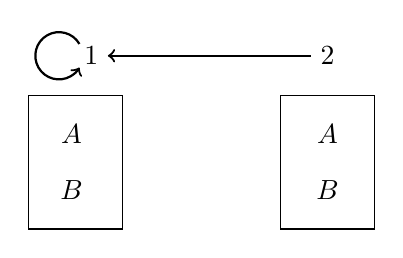
\begin{tikzpicture}
\node (atom1) at (0,1) {1};
\node (atom2) at (3,1) {2};
\node (atom3) at (-0.25,0) {$A$};
\node (atom4) at (3,0) {$\enot A$};
\node (atom5) at (-0.25,-0.7) {$\enot B$};
\node (atom6) at (3,-0.7) {$B$};
\draw[->, thick] (atom1)+(-0.15,0.15) arc (-330:-30:.3); 
%\draw[->, thick] (atom2)+(0.15,-0.15) arc (-150:150:.3); 
\draw[<-, thick] (atom1) -- (atom2);
\draw (-0.8,-1.2) rectangle (0.4,0.5);
\draw (2.4,-1.2) rectangle (3.6,0.5);
\end{tikzpicture}
\end{center}

\noindent Here is how to read the interpretation off from this diagram. It contains just two worlds, 1 and 2. The arrows between the worlds indicate the accessibility relation. So 1 and 2 both access 1, but neither 1 nor 2 accesses 2. The boxes at each world let us know which atomic sentences are true at each world: $A$ is true at 1 but false at 2; $B$ is false at 1 but true at 2. You may only write an atomic sentence or the negation of an atomic sentence into one of these boxes. We can figure out what truth-values the more complex sentences get at each world from that. For example, on this interpretation all of the following sentences are true at $w_1$:
\begin{itemize}
\item[]$A\eand\enot B$, $B\eif A$, $\Diamond A$, $\Box\enot B$
\end{itemize}
If you don't like thinking diagrammatically, then you can also present an interpretation like this:
\begin{itemize}
\item[$W$:]$1,2$
\item[$R$:]$\langle 1,1\rangle, \langle 2,1\rangle$
\item[]$\nu_{1}(A)=1, \nu_{2}(B)=0, \nu_{2}(A)=0, \nu_{2}(B)=1$
\end{itemize}
You will get the chance to cook up some interpretations of your own shortly, when we start looking at \emph{counter-interpretations}.

\section{A Semantics for System $K$}
\label{SemanticsK}

We can now extend all of the semantic concepts that you learnt in \emph{forall}$\meta{x}$ to cover ML:
\factoidbox{
\begin{itemize}
\item  $\meta{A}_1,\meta{A}_2, \dots \meta{A}_n\therefore\meta{C}$ is \textsc{modally valid} iff there is no world in any interpretation at which $\meta{A}_1,\meta{A}_2, \dots \meta{A}_n$ are all true and $\meta{C}$ is false.

\item $\meta{A}$ is a \textsc{modal logical truth} iff $\meta{A}$ is true at every world in every interpretation.

\item $\meta{A}$ is a \textsc{modal contradiction} iff $\meta{A}$ is false at every world in every interpretation.

\item $\meta{A}$ is \textsc{modally consistent} iff $\meta{A}$ is true at some world in some interpretation.
\end{itemize}
}
(From now on we will drop the explicit `modal' qualifications, since they can be taken as read.)

We can also extend our use of $\vDash$. However, we need to add subscripts again, just as we did with $\vdash$. So, when we want to say that $\meta{A}_1,\meta{A}_2, \dots \meta{A}_n\therefore\meta{C}$ is valid, we will write: $\meta{A}_1,\meta{A}_2, \dots \meta{A}_n\vDash_K\meta{C}$. Why did we choose the subscript $K$? Well, it turns out that there is an important relationship between system $K$ and the definition of validity we have just given. In particular, we have the following two results:
\begin{itemize}
\item If $\meta{A}_1,\meta{A}_2, \dots \meta{A}_n\vdash_K\meta{C}$, then $\meta{A}_1,\meta{A}_2, \dots \meta{A}_n\vDash_K\meta{C}$
\item If $\meta{A}_1,\meta{A}_2, \dots \meta{A}_n\vDash_K\meta{C}$, then $\meta{A}_1,\meta{A}_2, \dots \meta{A}_n\vdash_K\meta{C}$
\end{itemize}
The first result is known as a \emph{soundness} result, since it tells us that the rules of $K$ are good, sound rules: if you can vindicate an argument by giving a proof for it using system $K$, then that argument really is valid. The second result is known as a \emph{completeness} result, since it tells us that the rules of $K$ are broad enough to capture all of the valid arguments: if an argument is valid, then it will be possible to offer a proof in $K$ which vindicates it.

Now, it is one thing to state these results, quite another to prove them. However, I will not try to prove them here. If you are really interested, then you might want to look at any of the following: Garson's \emph{Modal Logic for Philosophers}; Priest's \emph{An Introduction to Non-Classical Logic}; Hughes and Cresswell's \emph{A New Introduction to Modal Logic}. None of these authors formulate their modal systems in quite the way we did, but it is not too hard hard to see how to translate their proofs of soundness and completeness over to our system. (The closest formulation is given by Garson, so the best place to start would be his \emph{Modal Logic for Philosophers}.)

For now, let's get more of a feel for this semantics by presenting some counter-interpretations. Consider the following (false) claim:
\begin{itemize}
\item[]
\begin{itemize}
\item[]$\enot A\vDash_K \enot \Diamond A$
\end{itemize}
\end{itemize}
In order to present a counter-interpretation to this claim, we need to cook up an interpretation which makes $\enot A$ true at some world $w$, and $\enot\Diamond A$ false at $w$. Here is one such interpretation, presented diagrammatically:
\begin{center}
\begin{tikzpicture}
\node (atom1) at (0,1) {1};
\node (atom2) at (3,1) {2};
\node (atom3) at (-0.25,0) {$\enot A$};
\node (atom4) at (3,0) {$A$};
\draw[->, thick] (atom1) -- (atom2);
\draw (-0.8,-0.6) rectangle (0.4,0.5);
\draw (2.4,-0.6) rectangle (3.6,0.5);
\end{tikzpicture}
\end{center}
It is easy to see that this will work as a counter-interpretation for our claim. First, $\enot A$ is true at world $1$. And second, $\enot\Diamond A$ is false at $1$: $A$ is true at $2$, and $2$ is accessible from $1$. So there is some world in this interpretation where $\enot A$ is true and $\enot\Diamond A$ is false, so it is not the case that $\enot A\vDash_K\enot\Diamond A$.


\section{A Semantics for System $T$}
\label{SemanticsT}

A few moments ago, I said that system $K$ is sound and complete. Where does that leave the other modal systems we looked at, namely $T$, $S4$ and $S5$? Well, they are all \emph{unsound}, relative to the definition of validity we gave above. For example, all of these systems allow us to infer $A$ from $\Box A$, even though $\Box A\nvDash_K A$.

Does that mean that these systems are a waste of time? Not at all! These systems are only unsound \emph{relative to the definition of validity we gave above}. (Or to use symbols, they are unsound relative to $\vDash_K$.) So when we are dealing with these stronger modal systems, we just need to modify our definition of validity to fit. This is where accessibility relations come in really handy.

When I introduced you to the idea of an accessibility relation, I said that it could be any relation between worlds that you like: you could have it relating every world to every world, no world to any world, or anything in between. That is how we were thinking of accessibility relations in our definition of $\vDash_K$. But if we wanted, we could start putting some restrictions on the accessibility relation. In particular, we might insist that it has to be \emph{reflexive}:
\begin{itemize}
\item $\forall wRww$
\end{itemize}
In English: every world accesses itself. Or in terms of relative possibility: every world is possible relative to itself. If we imposed this restriction, we could introduce a new consequence relation, $\vDash_T$, as follows:
\factoidbox{
$\meta{A}_1,\meta{A}_2, \dots \meta{A}_n\vDash_T \meta{C}$ iff there is no world in any interpretation \emph{which has a reflexive accessibility relation}, at which $\meta{A}_1,\meta{A}_2, \dots \meta{A}_n$ are all true and $\meta{C}$ is false
}
I have attached the $T$ subscript to $\vDash$ because it turns out that system $T$ is sound and complete relative to this new definition of validity:
\begin{itemize}
\item If $\meta{A}_1,\meta{A}_2, \dots \meta{A}_n\vdash_T\meta{C}$, then $\meta{A}_1,\meta{A}_2, \dots \meta{A}_n\vDash_T\meta{C}$
\item If $\meta{A}_1,\meta{A}_2, \dots \meta{A}_n\vDash_T\meta{C}$, then $\meta{A}_1,\meta{A}_2, \dots \meta{A}_n\vdash_T\meta{C}$
\end{itemize}
As before, I will not try to prove these soundness and completeness results. However, it is relatively easy to see how insisting that the accessibility relation must be reflexive will vindicate the $T$ rule:
\factoidbox{
\[\begin{nd}
\have[m]{m}{\Box \meta{A}}
\have[\, ]{n}{\meta{A}}\by{$T$}{m}
\end{nd}\]
}
To see this, just imagine trying to cook up a counter-interpretation to this claim:
\[
\Box \meta{A}\vDash_T \meta{A}
\]
We would need to construct a world, $w$, at which $\Box \meta{A}$ was true, but $\meta{A}$ was false. Now, if $\Box \meta{A}$ is true at $w$, then $\meta{A}$ must be true at every world $w$ accesses. But since the accessibility relation is reflexive, $w$ is accesses $w$. So $\meta{A}$ must be true at $w$. But now $\meta{A}$ must be true \emph{and} false at $w$. Contradiction!

\section{A Semantics for $S4$}
\label{SemanticsS4}

How else might we tweak our definition of validity? Well, we might also stipulate that the accessibility relation has to be \emph{transitive}:
\begin{itemize}
\item $\forall w_1\forall w_2\forall w_3 ((Rw_1w_2 \eand Rw_2w_3)\eif Rw_1w_3)$
\end{itemize}
In English: if $w_1$ accesses $w_2$, and $w_2$ accesses $w_3$, then $w_1$ accesses $w_3$. Or in terms of relative possibility: if $w_3$ is possible relative to $w_2$, and $w_2$ is possible relative to $w_1$, then $w_3$ is possible relative to $w_1$. If we added this restriction on our accessibility relation, we could introduce a new consequence relation, $\vDash_{S4}$, as follows:
\factoidbox{
$\meta{A}_1,\meta{A}_2, \dots \meta{A}_n\vDash_{S4} \meta{C}$ iff there is no world in any interpretation \emph{which has a reflexive and transitive accessibility relation}, at which $\meta{A}_1,\meta{A}_2, \dots \meta{A}_n$ are all true and $\meta{C}$ is false
}
I have attached the $S4$ subscript to $\vDash$ because it turns out that system $S4$ is sound and complete relative to this new definition of validity:
\begin{itemize}
\item If $\meta{A}_1,\meta{A}_2, \dots \meta{A}_n\vdash_{S4}\meta{C}$, then $\meta{A}_1,\meta{A}_2, \dots \meta{A}_n\vDash_{S4}\meta{C}$
\item If $\meta{A}_1,\meta{A}_2, \dots \meta{A}_n\vDash_{S4}\meta{C}$, then $\meta{A}_1,\meta{A}_2, \dots \meta{A}_n\vdash_{S4}\meta{C}$
\end{itemize}
As before, I will not try to prove these soundness and completeness results. However, it is relatively easy to see how insisting that the accessibility relation must be transitive will vindicate the $S4$ rule:
\factoidbox{
\[\begin{nd}
\have[m]{m}{\Box\meta{A}}
\have[\, ]{n}{\Box\Box\meta{A}}\by{$S4$}{m}
\end{nd}\]
}
To see this, just imagine trying to cook up a counter-interpretation to this claim:
\begin{itemize}
\item[]$\Box\meta{A} \vDash_{S4} \Box \Box \meta{A}$
\end{itemize}
We would need to construct a world, $w_1$, at which $\Box\meta{A}$ was true, but $\Box \Box \meta{A}$ was false. Now, if $\Box \Box \meta{A}$ is false at $w_1$, then $w_1$ must access some world, $w_2$, at which $\Box\meta{A}$ is false. Equally, if $\Box \meta{A}$ is false at $w_2$, then $w_2$ must access some world, $w_3$, at which $\meta{A}$ is false. We just said that $w_1$ accesses $w_2$, and $w_2$ accesses $w_3$. So since we are now insisting that the accessibility relation be transitive, $w_1$ must access $w_3$. And as $\Box\meta{A}$ is true at $w_1$, and $w_3$ is accessible from $w_1$, it follows that $\meta{A}$ must be true at $w_3$. So $\meta{A}$ is true \emph{and} false at $w_3$. Contradiction!

\section{A Semantics for $S5$}
\label{SemanticsS5}

Let's put one more restriction on the accessibility relation. This time, let's insist that it must be \emph{symmetric}:
\begin{itemize}
\item $\forall w_1\forall w_2(Rw_1w_2 \eif Rw_2w_1)$
\end{itemize}
In English: if $w_1$ accesses $w_2$, then $w_2$ accesses $w_1$. Or in terms of relative possibility: if $w_2$ is possible relative to $w_1$, then $w_1$ is possible relative to $w_2$. Logicians call a relation that is reflexive, symmetric and transitive an \emph{equivalence} relation. We can now define a new consequence relation, $\vDash_{S5}$, as follows:
\factoidbox{
$\meta{A}_1,\meta{A}_2, \dots \meta{A}_n\vDash_{S5} \meta{C}$ iff there is no world in any interpretation \emph{whose accessibility relation is an equivalence relation}, at which $\meta{A}_1,\meta{A}_2, \dots \meta{A}_n$ are all true and $\meta{C}$ is false
}
I have attached the $S5$ subscript to $\vDash$ because it turns out that system $S5$ is sound and complete relative to this new definition of validity:
\begin{itemize}
\item If $\meta{A}_1,\meta{A}_2, \dots \meta{A}_n\vdash_{S5}\meta{C}$, then $\meta{A}_1,\meta{A}_2, \dots \meta{A}_n\vDash_{S5}\meta{C}$
\item If $\meta{A}_1,\meta{A}_2, \dots \meta{A}_n\vDash_{S5}\meta{C}$, then $\meta{A}_1,\meta{A}_2, \dots \meta{A}_n\vdash_{S5}\meta{C}$
\end{itemize}
As ever, I will not try to prove these soundness and completeness results here. However, it is relatively easy to see how insisting that the accessibility relation must be an equivalence relation will vindicate the $S5$ rule:
\factoidbox{
\[\begin{nd}
\have[m]{m}{\Diamond \meta{A}}
\have[\, ]{n}{\Box\Diamond\meta{A}}\by{$S5$}{m}
\end{nd}\]
}
To see this, just imagine trying to cook up a counter-interpretation to this claim:
\[
\Diamond\meta{A} \vDash_{S5} \Box \Diamond \meta{A}
\]
We would need to construct a world, $w_1$, at which $\Diamond\meta{A}$ was true, but $\Box \Diamond \meta{A}$ was false. Now, if $\Diamond\meta{A}$ is true at $w_1$, then $w_1$ must access some world, $w_2$, at which $\meta{A}$ is true. Equally, if $\Box \Diamond \meta{A}$ is false at $w_1$, then $w_1$ must access some world, $w_3$, at which $\Diamond \meta{A}$ is false. Since we are now insisting that the accessibility relation is an equivalence relation, and hence symmetric, we can infer that $w_3$ accesses $w_1$. Thus, $w_3$ accesses $w_1$, and $w_1$ accesses $w_2$. Again, since we are now insisting that the accessibility relation is an equivalence relation, and hence transitive, we can infer that $w_3$ accesses $w_2$. But earlier we said that $\Diamond \meta{A}$ is false at $w_3$, which implies that $\meta{A}$ is false at every world which $w_3$ accesses. So $\meta{A}$ is true \emph{and} false at $w_2$. Contradiction!

In the definition of $\vDash_{S5}$, we stipulated that the accessibility relation must be an equivalence relation. But it turns out that there is another way of getting a notion of validity fit for $S5$. Rather than stipulating that the accessibility relation be an equivalence relation, we can instead stipulate that it be a \emph{universal} relation:
\begin{itemize}
\item $\forall w_1\forall w_2Rw_1w_2$
\end{itemize}
In English: every world accesses every world. Or in terms of relative possibility: every world is possible relative to every world. Using this restriction on the accessibility relation, we could have defined $\vDash_{S5}$ like this:
\factoidbox{
$\meta{A}_1,\meta{A}_2, \dots \meta{A}_n\vDash_{S5} \meta{C}$ iff there is no world in any interpretation \emph{which has a universal accessibility relation}, at which $\meta{A}_1,\meta{A}_2, \dots \meta{A}_n$ are all true and $\meta{C}$ is false
}
If we defined $\vDash_{S5}$ like this, we would still get the same soundness and completeness results for $S5$. What does this tell us? Well, it means that if we are dealing with a notion of necessity according to which \emph{every} world is possible relative to \emph{every} world, then we should use $S5$. What is more, most philosophers assume that the notions of necessity that they are most concerned with, like \emph{logical necessity} and \emph{metaphysical necessity}, are of exactly this kind. So $S5$ is the modal system that most philosophers use most of the time.

\practiceproblems

\problempart
Present counter-interpretations to the following false claims:
\begin{earg}
\item $\enot P \vDash_K \enot\Diamond P$
\item $\Box(P \eor Q)\vDash_K \Box P \eor \Box Q$
\item $\vDash_K \enot \Box (A\eand \enot A)$
\item $\Box A\vDash_K A$
\end{earg}

\problempart
Present counter-interpretations to the following false:
\begin{earg}
\item $\Diamond A\vDash_{S4} \Box\Diamond A$
\item $\Diamond A, \Box (\Diamond A \eif B)\vDash_{S4}\Box B$
\end{earg}

\problempart
Present counter-interpretations to the following false claims:
\begin{earg}
\item $\Box (M\eif O),\Diamond M\vDash_T O$
\item $\Box A\vDash_T \Box \Box A$
\end{earg}

